\documentclass{article}


%preamble
%required
%\usepackage{Sweave} %Integrates R code with LaTeX for creating dynamic reports
\usepackage{natbib}%Provides citation and bibliography support
\usepackage{amsmath}%Enhances mathematical typesetting capabilities.
\usepackage{textcomp}%among other things, it allows degrees C to be added
\usepackage{float}%Helps with precise figure placement using the [H] option.
\usepackage[utf8]{inputenc} % allow funny letters in citations 
\usepackage[nottoc]{tocbibind} %should add Re fences to the table of contents?
\usepackage{amsmath} % making nice equations 
\usepackage{listings} % add in stan code
\usepackage{xcolor}
\usepackage{capt-of}%allows me to set a caption for code in appendix 
\usepackage[export]{adjustbox} % adding a box around a map
\usepackage{lineno}
\linenumbers

% recommended! Uncomment the below line and change the path for your computer!
% \SweaveOpts{prefix.string=/Users/Lizzie/Documents/git/teaching/demoSweave/Fig.s/demoFig, eps=FALSE} 
%put your Fig.s in one place! Also, note that here 'Fig.s' is the folder and 'demoFig' is what each 
% Fig. produced will be titled plus its number or label (e.g., demoFig-nqpbetter.pdf')
% make your captioning look better
\usepackage[small]{caption}

\usepackage{xr-hyper} %refer to Fig.s in another document
\usepackage{hyperref}

\setlength{\captionmargin}{30pt}
\setlength{\abovecaptionskip}{0pt}
\setlength{\belowcaptionskip}{10pt}

% optional: muck with spacing
\topmargin -1.5cm        
\oddsidemargin 0.5cm   
\evensidemargin 0.5cm  % same as odd side margin but for left-hand pages
\textwidth 15.59cm
\textheight 21.94cm 
% \renewcommand{\baselinestretch}{1.5} % 1.5 lines between lines
\parindent 0pt		  % sets leading space for paragraphs
% optional: cute, fancy headers
\usepackage{fancyhdr}
\pagestyle{fancy}
%\fancyhead[LO]{Frederik Baumgarten}
%\fancyhead[RO]{Research Proposal}
% more optionals! %

\usepackage{graphicx}
\graphicspath{{/Users/frederik/github/PlantDeterminism/figures/}} % specify the path to your figures directory




\begin{document}
	
	
	% Format for a letter in "Ecology Letters"
	\title{Invest now, get paid later? Growth strategies to cope with environmental stress and benefit from extended growing seasons in a future climate %(my favourite)
		
		%dlDec18: Alternate title ideas:
		%Growth determinism/determinacy/habits in plants/woody perennials/trees: Limits and opportunities of species to time growth activities in a future climate. 
		
		%Growth determinacy in temperate trees: investing at the right time to cope with environmental stress and benefit from extended growing seasons in a future climate.
	} 
	
	\date{\today}
	\author{Frederik Baumgarten\textsuperscript{1,2}, Yann Vitasse\textsuperscript{2}, Sally?, Rob?, EM Wolkovich\textsuperscript{1}}
	\maketitle
	
	$^1$ Department of Forest and Conservation, Faculty of Forestry, University of British Columbia, 2424 Main Mall
	Vancouver, BC Canada V6T 1Z4. \\
	
	$^2$  Swiss Federal Institute for Forest, Snow and Landscape Research WSL, Zürcherstr. 111, Birmensdorf 8903, Switzerland\\
	
	Corresponding Author: Frederik Baumgarten; frederik.baumgarten@ubc.ca \\
	Journal: Perspective in Ecology Letters
	
	%Full word count: \\
	%Summary word count: \\
	%Introduction word count: \\
	%Materials and Methods word count: \\
	%Results and figure legends word count: \\
	%Discussion word count: \\
	
	%werwolve: how is tree growth impacted by climate change? 1) by extreme events and 2) by an extended growing season? 
	%baby: better predictions of when environmental factors are influencing growth taking into account the phenological sequence of a species
	%silverbullet: concept of determinism
	
	
	

	
\section*{Abstract} %150 words
		With increasing latitude, plants are confined to a shrinking ‘time window of opportunity’ set by low temperatures (frost) and water restrictions (drought). For trees, the fundamental questions of when and how much growth occurs within this window, are still poorly addressed and their answers are more pressing than ever to predict biomass production and carbon sequestration in the current and future climate. Much progress has been made to reveal the relationships of environmental drivers with growth and development, particularly the physiological effects of low and high temperature thresholds as well as decreasing cell pressure (turgor) under limiting soil water availability. \\
		Yet, environmental conditions do not solely explain if a plant during the active season is growing or not. An often-overlooked factor is the phenological sequence – the developmental stages and transitions set by the genetic programming of a plant that manifests in species-specific growth patterns/habits. This internal schedule has the power to impose switches in physiological activity e.g. from structural vegetative growth to reproduction (such as fruit ripening), storage accumulation and inducing senescence \textit{despite} growth-promoting conditions.\\
		Here, we revise the old concept of (in-)determinism: the ability of trees to preform tissue as an investment for next year’s growth that will overwinter in buds vs. a strategy that additionally relies on the continuous activity of the apical meristem throughout the growing season (neo-formed tissue). We propose that 1) determinate species may be more resistant and resilient to environmental stressors (e.g. drought) and 2) the higher the degree of indeterminacy in a species, the greater its capacity/potential to profit from extended growing seasons. Consequently, the question of how much carbon will be sequestered in a future climate might depend not only on abiotic factors like water availability, temperature extremes and the length of the growing season, but also on the degree of determinacy set by a species' intrinsic genetic programming.\\
		
			\textbf{Keywords}: plant growth, tree phenology, shoot extension, indeterminate growers, carbon sequestration, growing season length, drought, genetic programming, phenotypic plasticity
			\newpage
			
\section*{Introduction}
	
	\subsection*{Timing of investments}
		Investing at the right time is of crucial importance for the survival and fitness of plants. While in tropical ecosystems a continued production of tissue can be both possible and advantageous, in most other regions strategies that rely on growth from stored reserves and pre-build tissue are widely common. %The rapid canopy formation of deciduous trees in spring of temperate forests is such an example. However, canopy duration is a poor predictor of when growth and therefore carbon sequestration occur

	\subsection*{Seasonality of temperature and soil moisture}
		The further one travels from the equator towards the poles, the tighter plants are confined to a shrinking ‘time window of opportunity’ set primarily by low temperatures. Below c. 5°C  metabolic activity slows down to an extend where growth and development comes to a halt \citep{schenkerPhysiologicalMinimumTemperatures2014, rossiCriticalTemperaturesXylogenesis2008, kornerWinterCropGrowth2008}. More importantly, freezing temperatures can cause severe damages to plant tissue if exposed at the wrong time of development, e.g. after leaf unfolding or prior to fruit maturation \citep{baumgartenNoRiskNo2023a}. While annual plant species accommodate their entire life cycle within this window, perennial plants are forced to split their growing phase into annual chunks with periods of activity alternating with a period of rest (dormancy). This is referred to as intermittent or rhythmic (as opposed to continuous) growth. \\
		
		During the active growing season high temperatures can also reduce plant activity and development, ultimately to the point where meristems fail to produce new tissue and protein structures fall apart if species-specific thresholds are exceeded \citep{osullivanThermalLimitsLeaf2017}. High temperatures increase the evaporative demand of plants which in turn decreases the water status (water potential) along the entire root-to-shoot-continuum. Trees are able to lift water to great heights, but meristems are not able to divide cells under too low cell pressure (turgor), which explains the physical limits to tree height \citep{kochLimitsTreeHeight2004} and why trees mainly grow at night, when transpiration stops and cell turgor relaxes \citep{zweifelWhyTreesGrow2021}. Of course meristematic activity completely ceases under limited soil water availability --- a major reason why trees in many regions grow only  a fraction of days within the potential thermal growing season \citep{etzoldNumberGrowthDays2021}. Figure \ref{fig:fig_1xxx} shows these temperature and soil moisture limitations as 'environmental filters', narrowing the window of opportunity where potential growth could happen. \\
		
		\subsection*{Internal programming of plants}
		Given our developed physiological understanding on how growth is controlled by environmental factors, namely temperature and soil moisture availability, one could think that predictions about when and how much trees are growing in a current and future climate should be fairly simple to make. However, this is not the case, in particular for predictions with extended climatic growing seasons \citep{zohnerHowChangesSpring2021}. It seems that environmental variables alone are not sufficient to capture the dynamic and extend of biomass production and therefore carbon sequestration.  Here we propose the framework for an additional factor to consider: internal growth control - the genetically fixed developmental program that can dictate not to grow \textit{despite} of favourable environmental conditions.\\
		
		While plants have evolved many mechanism to tolerate or avoid such potentially harmful conditions by specialized morphological adaptations, most species, even in the tropics cope with fluctuating temperature and moisture regimes by temporally escaping these conditions. This involves the progression of a dormancy cycle and the timing and prioritization of life history events (phenology). Plants outside the agricultural context rarely maximize biomass production \citep{kornerConceptsEmpiricalPlant2018}. Rather they are selected for survival to increase their fitness which is tightly linked to their intrinsic programming (or phenological sequence) which imposes abrupt switches in resource allocation from vegetative growth to reproduction (flowering, fruit maturation) and storage (REF). Figure \ref{fig:fig_1xxx} shows these additional "internal filters" eventually narrowing down the window in which growth can effectively occur.\\
		
		
		%Here, we....point to future directions
		
								\begin{figure}
								\centering
								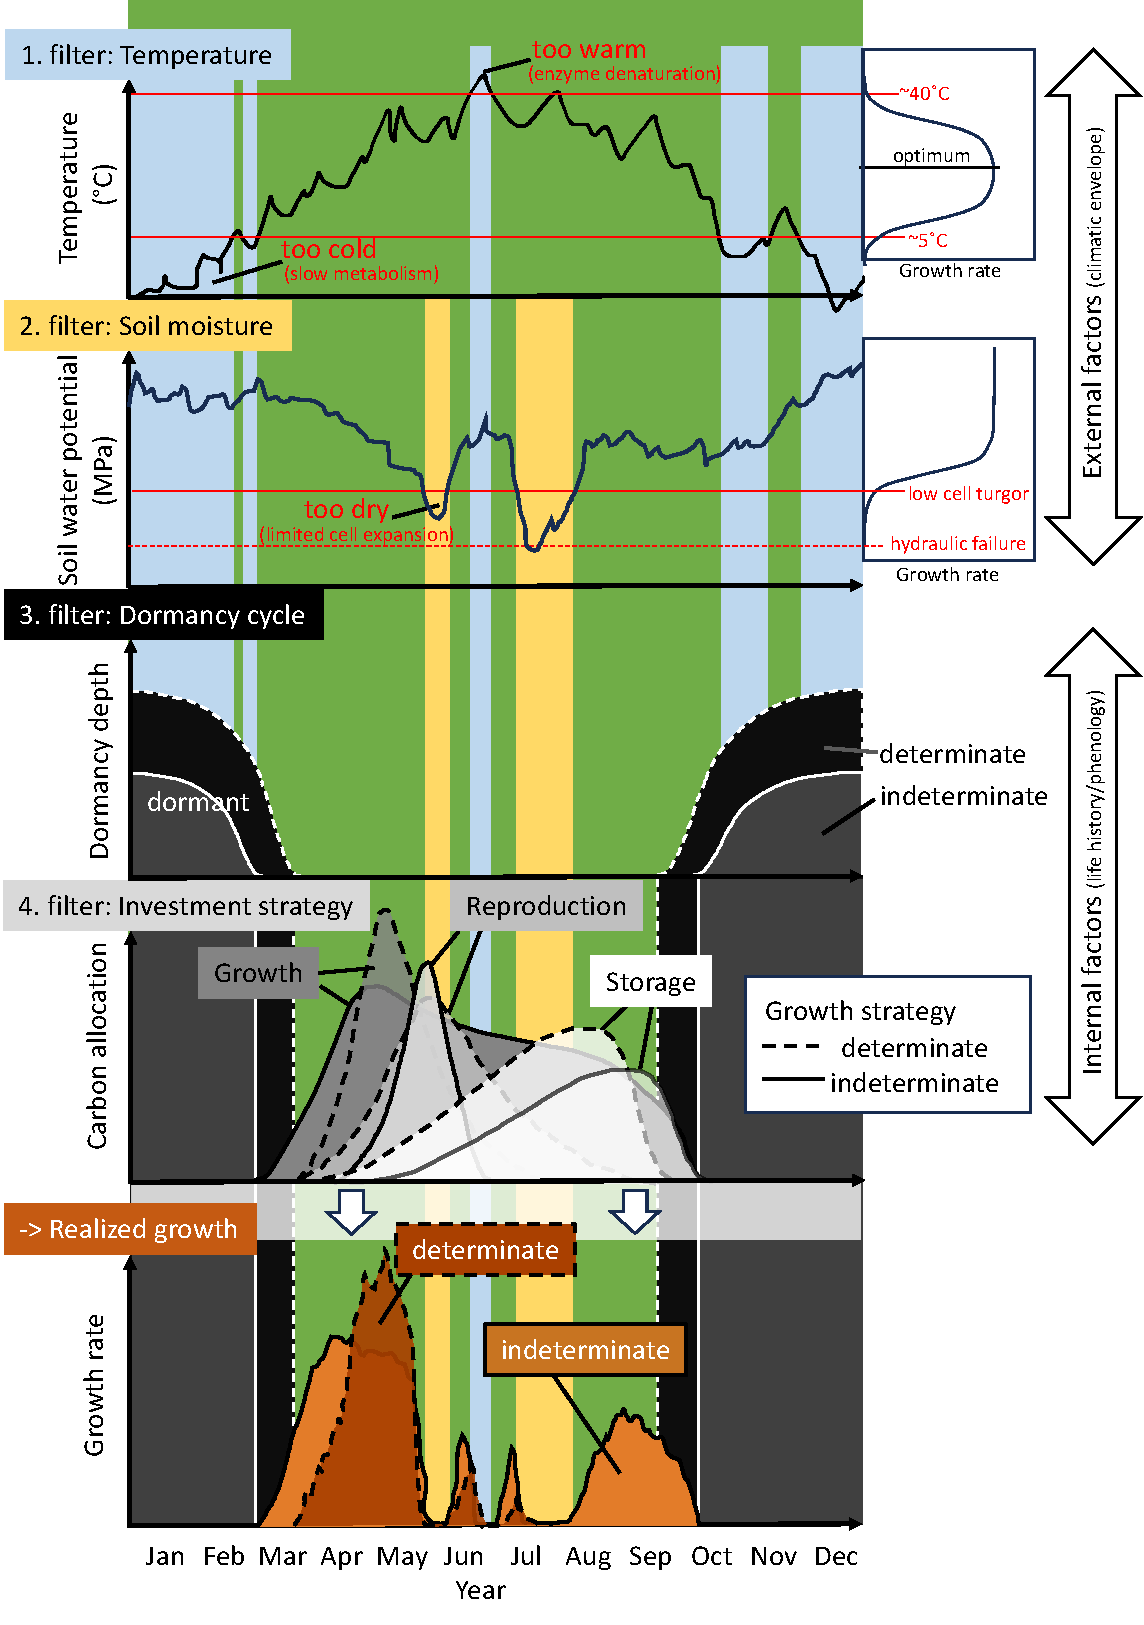
\includegraphics[width=0.9\textwidth]{Fig_1_V6.pdf} 
								\caption{Schematic overview of the discrepancy between the potential growing season and the effectively realized vegetative growth. Environmental factors like temperature and soil moisture, exceeding growth-promoting thresholds can be seen as filters that narrow the window of opportunity available for vegetative growth. The species-specific life history cycle (phenology) can further impose another filter by imposing a dormancy cycle and prioritizing developmental processes other than vegetative growth (e.g. flowering, fruit maturation and storage). }
								\label{fig:fig_1xxx}
							\end{figure}

	
\section*{The concept of (in)determinate growth}
The topic of growth strategies and habits has a long history in science, spanning the fields of genomics, physiology and ecology across the animal and plant kingdom. At its core lays the concept of determinacy --- the classification of organisms to either reach a fixed size with adulthood or to continue to grow throughout their lifetime. Like mollusks, fish and reptiles, plants add to their primary bodies as long as they live and are therefore considered 'indeterminate growers' \citep{ejsmondHowTimeGrowth2010}. Various terms emerged to describe this fundamental phenomenon at different spacial and temporal scales, e.g. from a cell to an organism and from a season to a whole lifetime \citep{mcdanielInductionDeterminationDevelopmental1992a, karkachTrajectoriesModelsIndividual2006}. \\

In annual plants, growth ends with the production of flowers to form fruits and seeds: a signal in the apical meristem causes a sudden switch in resource investment from vegetative growth to building a reproductive structure with no point of return, ringing in the end of its life-cycle. In contrast, most perennial plant species and trees in particular, build flowers on lateral buds to enable the seasonal production of offsprings while the vegetative structure keeps expanding. \\

Within one growing season, however, trees exhibit a strategy of determinacy (see Figure \ref{fig:fig_2xxx}): Most tree species prebuild part or their entire canopy in the previous year, overwintering in hardened buds to be 'ready to go' when spring arrives. Once the canopy is unfolded within a few days to weeks many species sustain their primary growth activity by hormonal suppression of the apical meristems for the rest of their growing season (paradormancy, \citep{langEndoParaEcodormancy1987}. This is contrasted by some species that continue to produce new tissue ontop of the preformed one in some cases stretching their growth period far into autumn until low temperature force them to stop. In summary, determinacy in trees refers to the ability to:\\
a) preform tissue as a future investment that is ready to be deployed in spring with sustained growth thereafter (determinate strategy)\\
b) maintain a somewhat constant growth activity (or activity bursts) by forming new tissue during the growing season (indeterminate strategy)\\

While this concept is often presented as dichotomous (\cite{kozlowskiGrowthControlWoody1997, lechowiczWhyTemperateDeciduous1984a}, but see \citet{kikuzawaLeafSurvivalWoody1983}), with species exhibiting either one extreme or the other, they more likely exist along a gradient with numerous intermediate forms. For example many oak species - considered determinate growers, exhibit a second flush and many species gradually become more determinate as they mature \citep{borchertConceptJuvenilityWoody1976, heuretOntogeneticTrendsMorphological2006}.
	
	
								\begin{figure}
								\centering
								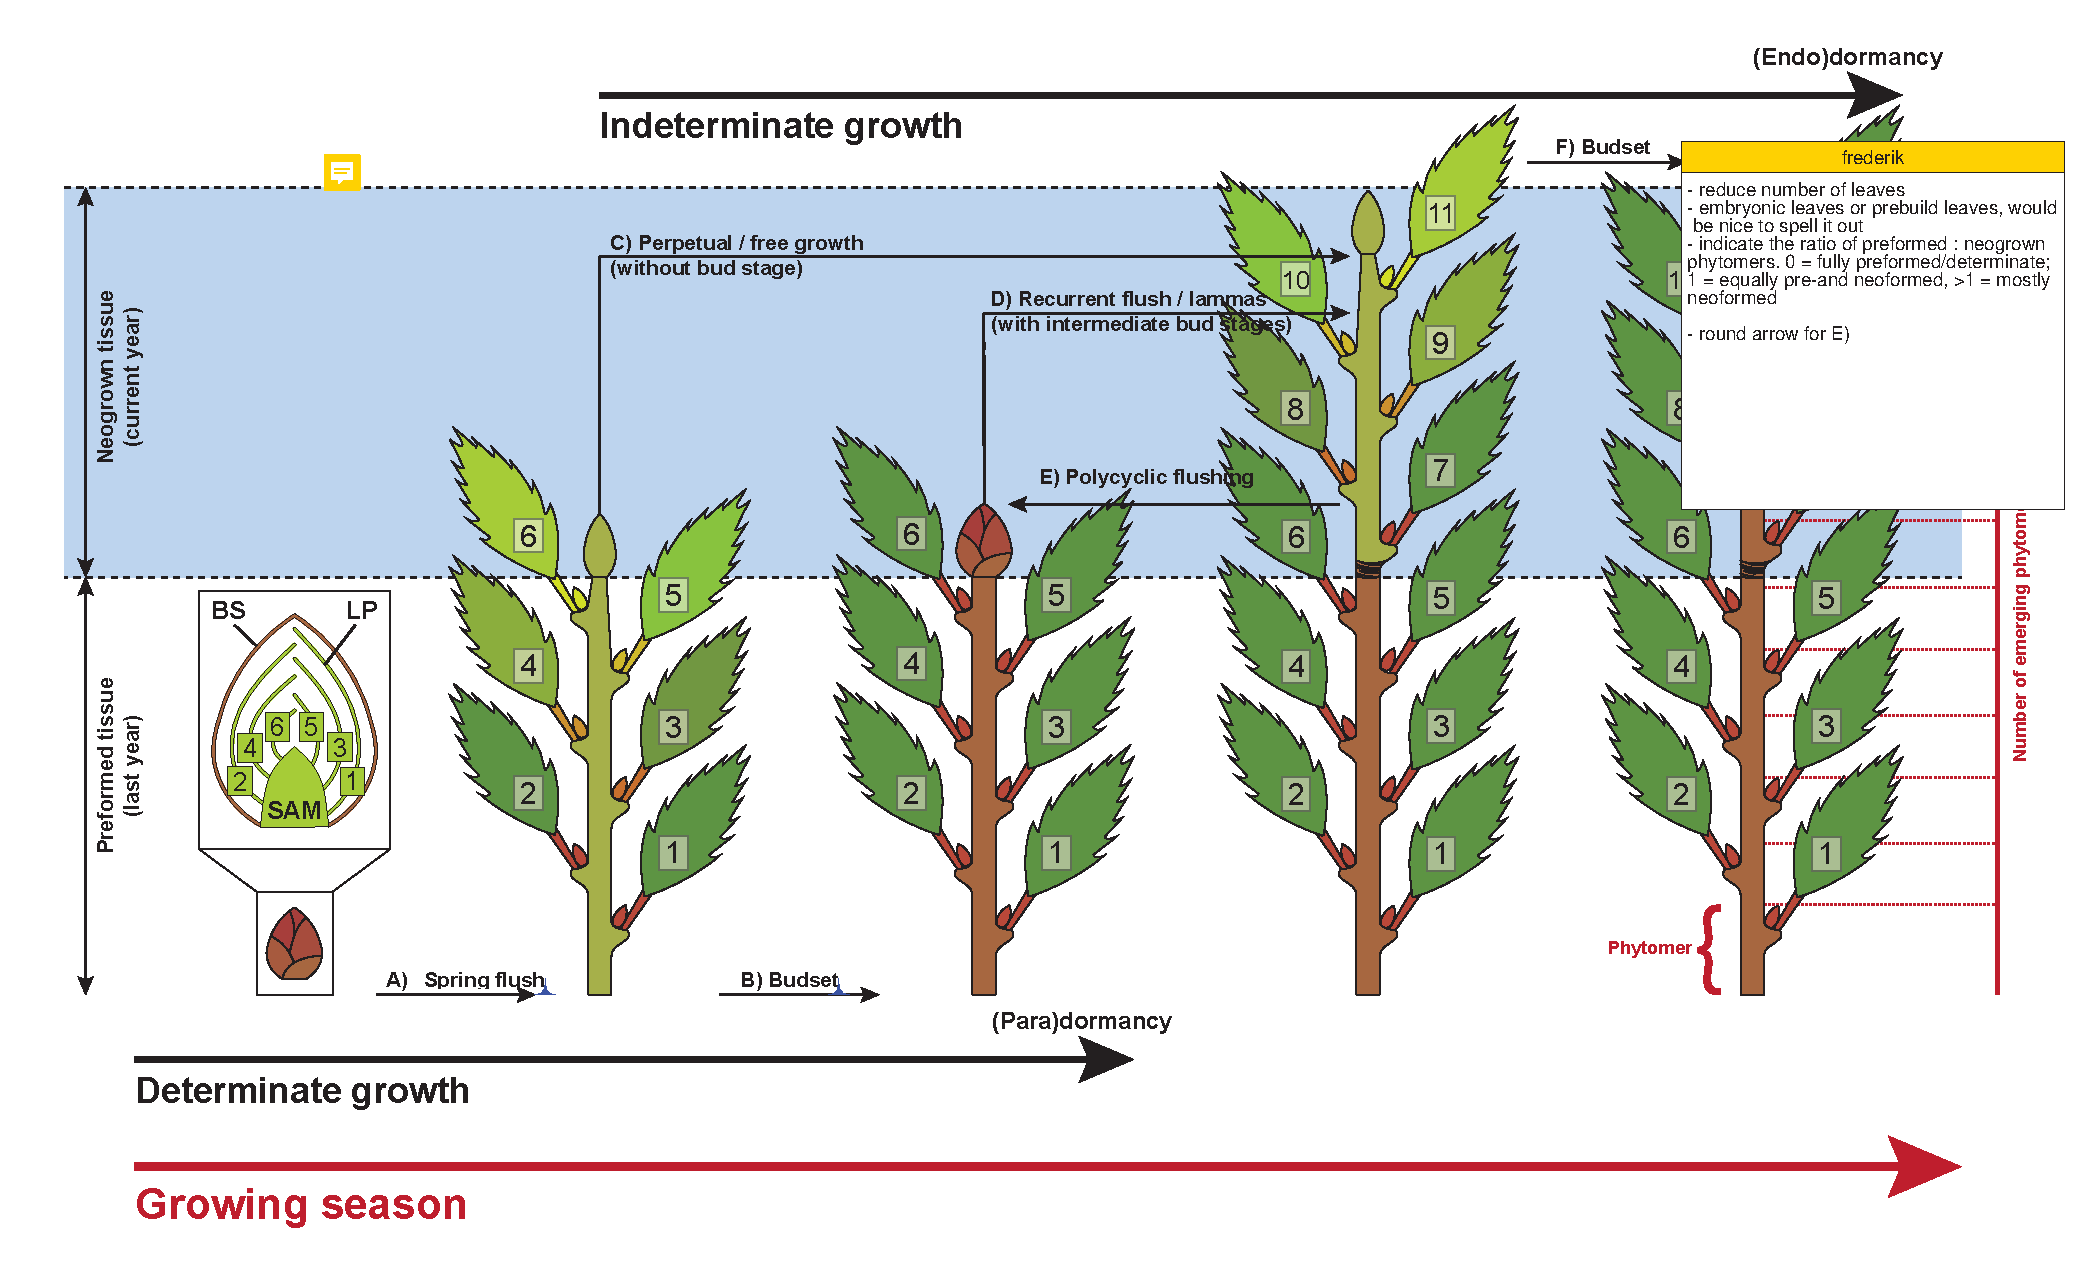
\includegraphics[width=1.1\textwidth]{determinismFigure_FB.pdf} 
								\caption{Determinate and indeterminate growth within one growing season. Commonly all tree species deploy buds during their first spring flush from prebuild and overwintering leaf primordia (A). Determinate growing species set bud (B) that are under hormonal suppression to sustain any further activity of the shoot apical meristem (paradormancy). Indeterminate growing species continue to produce new tissue directly (C) or through one (D) to several (E) intermediate bud stage(s). Finally all species set their bud (F) and enter full dormancy (endodormancy). Shoot apical meristem (SAM); Bud scale (BS); leaf primordia (LP). The basic unit of a shoot is the phytomer which is composed of a node, a leaf, the axillary bud and an internode.}
								\label{fig:fig_2xxx}
								\end{figure}
	
\section*{Control mechanisms/What controls/drivers of determinism}
Altough a century of studying growth habits has passed we still have very little understanding of when and why trees exhibit a certain degree of (in)determinsm in their growth strategy. To a large extend this is probably due to the variable environmental conditions within and between years as well as among sites and individuals that complicates the separation of factors influencing or driving shoot elongation and for that matter other meristematic activity.

Indeed there is some evidence, that under favorable conditions, particularly soil moisture availability, stretching into the growing season prolongs the period of shoot elongation or permitting a second flush, also known as lammas growth or "Johannitrieb" (see Figure \ref{fig:fig_2xxx}). This indicates that shoot growth may come to a halt because the demand for water, supporting a growing leave area, cannot be met. Since above and below-ground meristem experience large differences in temperature, the higher growth rate of shoots may soon result in an imbalanced root-shoot-ratio that can only be overcome by sustaining growth of the apical meristems until root growth has caught up to reach the supply capacity. A high evapotranspiration or a drying soil might have the same effect. Such a "stop-and-go" behavior of the apical meristem as a  consequence of lower growth rates in roots could explain the poly-cyclic flushing patterns observed in some species \cite{girardPolycyclismFundamentalTree2011}.\\

This latter mechanism is also supported by experimental data. Artificial reduction of the leaf area caused terminal buds to keep growing until the original leaf area was re-established \citep{borchertSimulationRhythmicTree1973}. Similarly many species produce new shoots after a damaging spring frost or after severe herbivory in order to rebuild their canopy. \\

However, this perspective suggests that the environment can completely flip a species' strategy --- but this is not the case. While manipulations on root:shoot ratios proof a certain plasticity of the apical shoot meristem to adjust leaf area after disturbance, we still observe distinct growth patterns when environmental conditions remain favorable . Hence, there must be an underlying internal program that sets the potential of how trees grow and explains the variation of growth habits among species we observe in the same environmental conditions (see Table XX for a list of species and their main growth strategy). 

latitudinal gradients and population differences within a species...Sally could help here
	c) these are fundamental trade-offs --- both successful and co -occur in communities
	successional stage, ontogeny, life span, evolution
	
	we should talk also about some downsides of the indeterminate strategy. e.g. faster turnover, increased exposure to risky climate, 
	
	...but will both still be successful with CC?
	
\section*{The role of determinism with climate change}
Climate change is extending the growing season length while at the same time increasing the risk for severe drought \citep{haoChangesSeverityCompound2018} and presumably also late spring frost events in many regions worldwide \citep{zohnerLatespringFrostRisk2020}. How are these potential benefits and threads linked to a species strategy, specifically to the degree of determinism? Which strategy profits most from an extended growing season length and which one is flexible enough to rearrange their phenological cycle to withstand increased environmental stress. And which one comes with more biomass production and C sequestration? We propose that the degree of determinism is an important trait largely controlling the responses of trees in a future climate illustrated in Figure \ref{fig:fig_4xxx}. 

			\subsection*{Growing season extended}
Spring warming has undoubtedly advanced the onset of leaf emergence by up to a month compared to pre-industrial times \citep{vitasseGreatAccelerationPlant2022b}. In contrast autumn phenology of growth and leaf senescence has not delayed as one could predict from environmental conditions (REF). In fact, the phenological sequence is observed to shift as a whole towards spring (REF), not necessarily leading to increased biomass production during longer growing seasons \citep{zaniIncreasedGrowingseasonProductivity2020b}. We hypothesize that only determinate growing species shift their growth in such a way with minimal changes in overall productivity. In contrast, indeterminate growing species are able to extend their growing season in both directions, leading to an increased productivity in a future climate (Figure \ref{fig:fig_4xxx}). 

			\subsection*{The risk of extreme events}
The downside of a strategy to maximise biomass production is the increased risk of exposure to extreme climatic events. Indeterminate species are often pioneers (REF) that are among the first to leaf-out and among the last to shed their leaves --- occasionally as a result of a freezing event. In addition a substantial part of their growth period falls into summer with increased risk of drought (Figure \ref{fig:fig_4xxx}). Therefore, we hypothesize that the conservative strategy of determinate growing species largely escape from unfavourable growing conditions by placing their growth activities between the last spring frost and the increasing water shortages in summer, with relatively large safety margins. As a consequence productivity shows little between year variation and will largely remain constant in a future climate. However, once hit by an extreme event, determinate growing species might not recover easily. Even if leaves are shed to prevent further damage, the loss of the canopy, which is rarely replaced in determinate species after summer, will contribute to a lower fitness and reserve pools. In contrast, the flexible growth schedule of indeterminate growing species may allow to 1) produce tissue better adapted to harsh environmental conditions as it is formed in the current season - even if that means no additional growth and 2) catch up and compensate later in the season by another productivity boost. \\

We argue that new opportunities and challenges with climate change will increasingly disrupt the phenological cycle of trees, favoring those who are more plastic in rearranging their activities by resuming growth, reproduction and/or storage filling later in the year, thereby recovering from and compensating for some stress-induced damages and losses. Future climate will therefore likely intensify the competition among co-occurring species and might re-assemble forest communities increasingly composed of species adopting an indeterminate growth strategy.

			Figure \ref{fig:fig_3xxx} shows an example figure.
	
								\begin{figure}
								\centering
								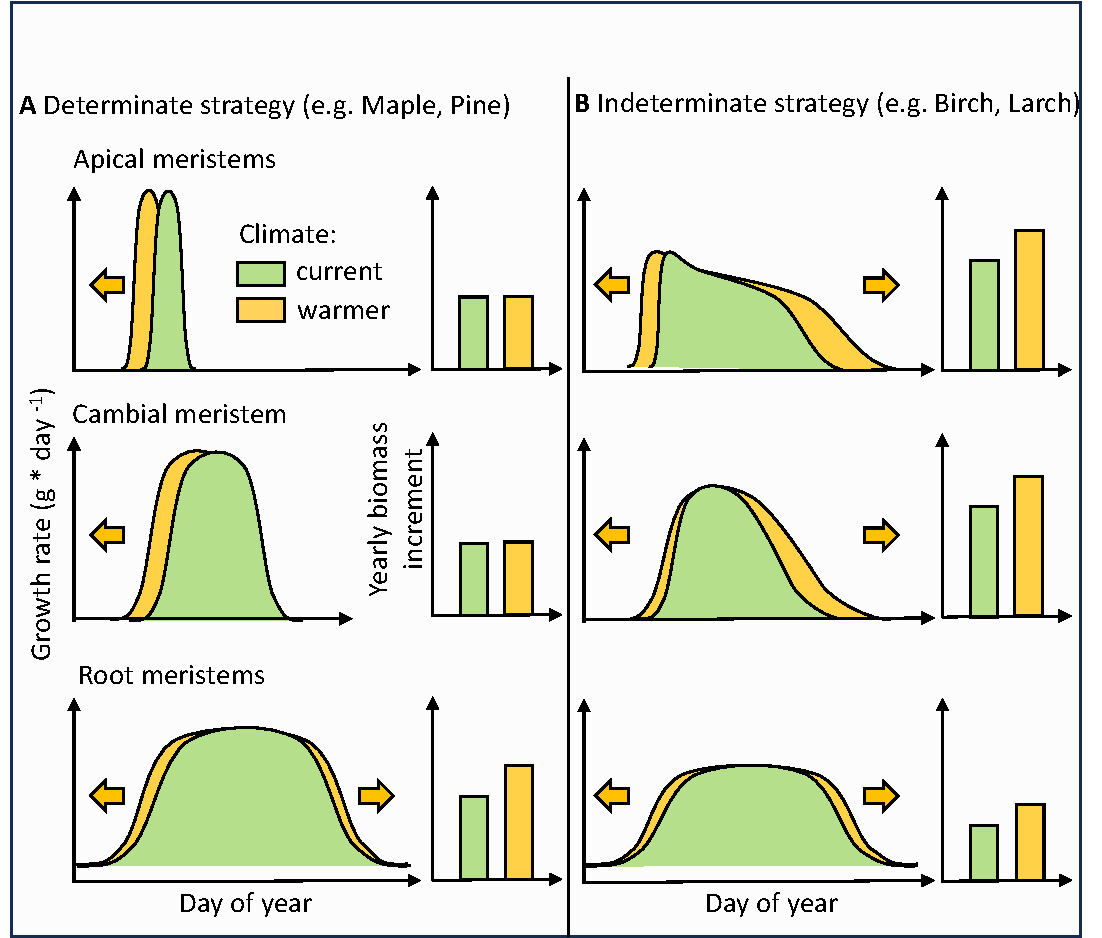
\includegraphics[width=0.9\textwidth]{Fig_3_V3.pdf} 
								\caption{Hypothesized predictions of growth rates for the three major meristems (apical, cambium and root) classes of trees under current and warmer climates following an extreme determinate (A) and indeterminate (B) growth strategy. The area under the curve is summarized as yearly biomass increment in the respective bar-plot. Arrows indicate the shift of growth phenology under warmer climate conditions. Root meristems appear to be purely temperature-opportunistic for both strategies, even growing during warm winter spells. The indicated genera were observed to showcase the illustrated trends. The responses of these two contrasting growth strategy might apply not only to different tree species but also within a population (e.g. along environmental gradients) and even within an individuum as it transitions from the junvenile to the adult stage (ontogeny).}
								\label{fig:fig_3xxx}
							\end{figure}
	
								\begin{figure}
								\centering
								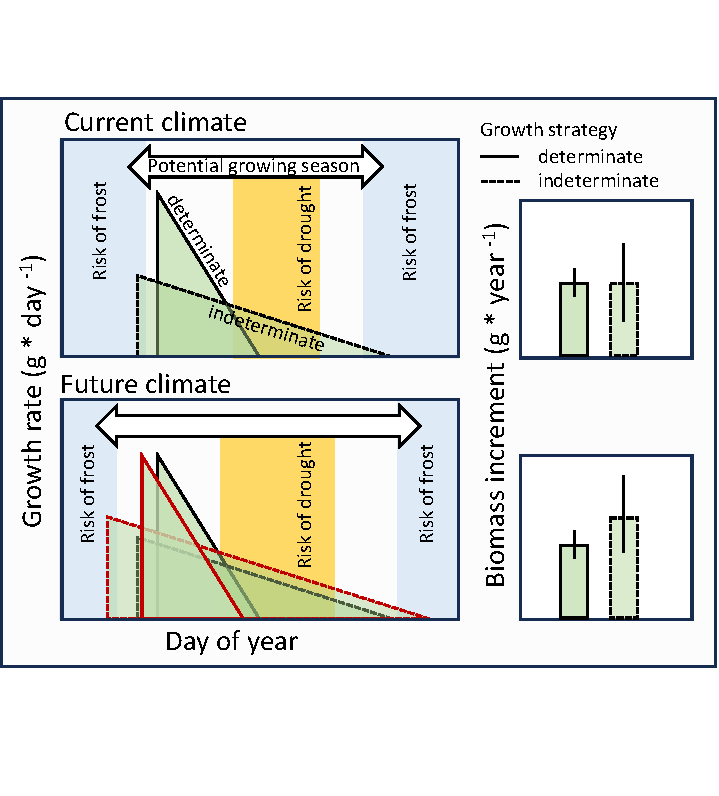
\includegraphics[width=0.9\textwidth]{Fig_4_V1.pdf} 
								\caption{Hypothesized predictions of growth rates under current and future climate for determinate and indeterminate growing species. Note that the indeterminate strategy is more exposed to the risk of frost and drought events while the determinate strategy condenses most growth within a rather safe period. In the current climate the indeterminate strategy is in balance with benefiting from the full climatic growing season in some years with some drawback in other years, resulting in the same mean yearly biomass increment, but with a higher variation; right box). In a future climate the indeterminate strategy might benefit exceedingly from longer growing seasons, resulting in an overall higher mean annual biomass increment compared to determinate growers.}
								\label{fig:fig_4xxx}
							\end{figure}
	\pagebreak
\section*{Future directions}
The fundamental questions regarding the timing and duration of growth remain and are more pressing than ever: When and how much is growth and therefore carbon sequestration most impacted by climate extremes? Moreover, we must question the potentials and limits of trees to adapt --- are they plastic enough to extend their growing period in a climate with prolonged seasons? Or are they bound to follow an internal program in which growth and development occurs within narrow, fixed temporal boundaries? 

\subsection*{Role of determinacy with climate extremes and prolonged growing seasons}
The concept of growth determinacy could play an important role in answering these questions and improve our predictions of future tree growth and performance. Specifically, how much degree of (in)determinism allows to escape periods of increased risk of environmental stress while being versatile enough to resume metabolic activities to repair damaged structures, restore reserves and eventually compensate for previous losses during the same season. Assessing the trade-off between buffering extreme events and exploiting a longer growing season will likely contribute to our understanding of how forest communities will assemble over the course of this century.\\

Going forward, we need to identify the plasticity of the trait of exhibiting indeterminate growth under different environmental conditions and the genetic programming of a species and to what extend the latter prioritizes the former. Namely, across species and populations and involving different fields from genomics to physiology and ecology. Moreover, we need to test how universal the concept can be applied/holds true across different meristems and resource allocation. %Lizzie: here I am not sure how to make the thing with resource allocation more clear. To me the strategy of (in)determinism already incorporates the allocation problem, e.g. a determinate species will switch sooner from vegetative growth to reproduction and storage, but perhaps this needs to be stated more clearly somewhere...

\subsection*{Patterns across meristems}
Although (in)determinate growth is mainly associated with the activity of the shoot apical meristem, a similar pattern or concept might be found in the cambium as well to ensure a timely switch from vegetative growth to reproductive and storage investments. In fact, also cambial cells produce several cohorts of precursor cells with differentiation and lignification being completed at a much later stage only \citep{valdovinos-ayalaSeasonalPatternsIncreases2022}. Hence the number of initial cells divided at the beginning largely determines the amount of total xylem produced \cite{lupiXylemPhenologyWood2010}. In this case, primary growth reflects or at least influences the overall growth performance of an individual, integrated across all above-ground meristems. The low predictive power to estimate the end of wood formation in autumn reported by several studies \cite{buttoComparingCellDynamics2020} indeed points to a mechanism that stem growth in many tree species ceases despite of ongoing favourable conditions and a  green canopy \cite{arendStemGrowthPhenology2024}.\\

Regarding below-ground meristems, roots seem to follow a much more opportunistic strategy with indeterminate growth potentially occuring throughout the year. Warming experiments using Rhizotrones have shown that roots can grow even in mid-winter if temperature allow it \cite{lyfordControlledGrowthForest1966}, suggesting that roots do not enter a state of dormancy \cite{radvilleRootPhenologyChanging2016}. To what extend asyinchrony between above and below-ground meristems occur as a result of different tissue temperatures, root:shoot imbalances or genetically fixed investment strategies remain unresolved\cite{abramoffAreBelowgroundPhenology2015, makotoSynchronousAsynchronousRoot2020}.\\

 Future studies should therefore link the temporal dynamics of primary (apical and root) and secondary (cambial) meristems. Correlating annual tree rings with shoot increments could reveal such a common pattern, if accounting for when interannual shoot segments (phytomers) were produced, e.g. separating preformed from neogrown tissue (REF Günter?). Revealing the patterns of when different meristems are active will likely contribute to a theoretical framework of temporal carbon allocation dynamics.

	

	gene/hormones (1-2 para) % Here I need to read some refs for input. 
	
	bii) Evol. history (end on metric fortshadowing) % @Lizzie: Here I dont know what to do at the moment...happy for some input
	
	
	\subsection*{Metrics of determinacy}
	To address these questions we need better metrics to quantify the degree of determinacy, moving beyond a dichotomous classification system. We propose several metrics from best to acceptable, with increasing spatial scale: \\
	
	(1) n leaves  EOS /n leaves primordia in buds SOS. Values higher than 1 indicate an increasing degree of indeterminate growth \\
	
	(2) direct measures of shoot elongation and/or xylogenesis (micro-cores) at high temporal resolution (e.g. bi-weekly) to assess the temporal dynamics of apical and cambial activity\\
	
	(3) dendrometers as a proxy for the temporal dynamic of xylem and phloem formation \\
	
	(4) Using observations of 'second flushes' in large databases (e.g. US national forest network). \\
	
	(5) Patterns and fluctuations of canopy growth detected from drones or satellites using Lidar or spectral techniques.
	

	

	
\section*{Acknowledgments}
	Justin Ngo for the help in illustrating
	


	
	

	
	\pagebreak
	

	\newpage
\section*{stuff I did't find place yet}

	
If experiments are conducted in conditions with unlimited soil moisture and under similar temperature regimes, then the dynamics of growth responses can be comparable among species and reveal their potential in deploying indeterminate growth. Under natural conditions with common soil moisture and associated turgor limitations it is currently hard to tell if trees cease growth because of a response to the environment or because of switches in resource allocation. 

 Grow fast die young...
 
 Even in grasslands an earlier onset of growth is associated with an earlier stop under climate warming \cite{mohlGrowthAlpineGrassland2022a}
	
indeterminate species are often early successional ones \citep{marksRelationExtensionGrowth1975, boojhGrowthStrategyTrees1982}

	
	must include: \cite{iwasaOptimalGrowthSchedule1989}
	\newpage
	
	\bibliography{refs_determinism}
	\bibliographystyle{ecolett}
	
	
	
\end{document}






